\begin{frame}
	\titlepage
\end{frame}

\begin{frame}{平面曲线的曲率}
	\linespread{1.5}
	\begin{columns}
		\column{.5\textwidth}
			\vspace{-2cm}
			\begin{itemize}
		      \item {\bf 平面曲线的曲率概念}
		      \item {\bf 曲率的计算公式}
		      \item {\bf 曲率圆与曲率的应用}
		    \end{itemize}
		\column{.5\textwidth}
			\vspace{2cm}
			\resizebox{!}{5cm}{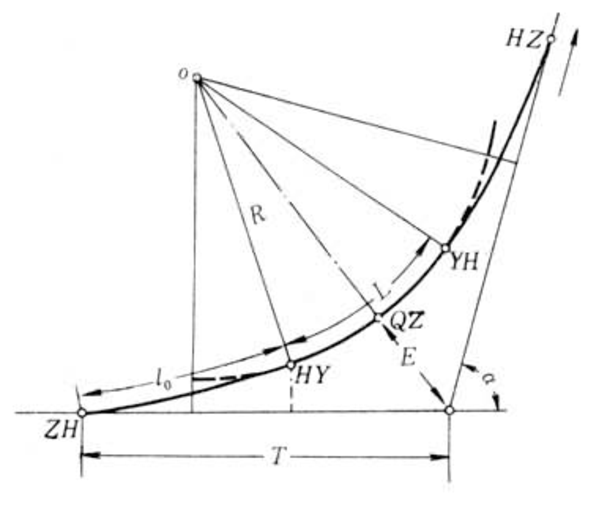
\includegraphics{./images/tcs.pdf}}
	\end{columns}
\end{frame}

\begin{frame}{铁路的设计}
	\linespread{1.2}
	\begin{center}
		\resizebox{!}{7cm}{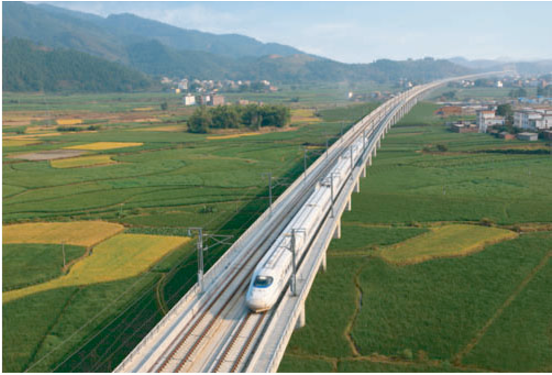
\includegraphics{./images/rw1.pdf}}
	\end{center}
\end{frame}

\begin{frame}{复习与回顾}
	\linespread{1.5}
	\ba{如何刻画一条平面曲线的几何特征?}
	
	\begin{enumerate}
	  \item {\bf 切线斜率:}一阶导数
	  \item {\bf 凹凸性:}二阶导数
	  \item {\bf 长度:}弧微分\pause
	  \item {\bf 弯曲程度:}{\b 曲率}
	\end{enumerate}
\end{frame}



%=================================================

\section{曲率}

\subsection{曲率的概念}

\begin{frame}{曲率}
	\linespread{1.2}
	\centerline{\ba{如何刻画曲线的弯曲程度?}}
	\pause
	\begin{columns}
		\column{.5\textwidth}
			\begin{center}
				\vspace{-1em}
				{\resizebox{!}{5.5cm}{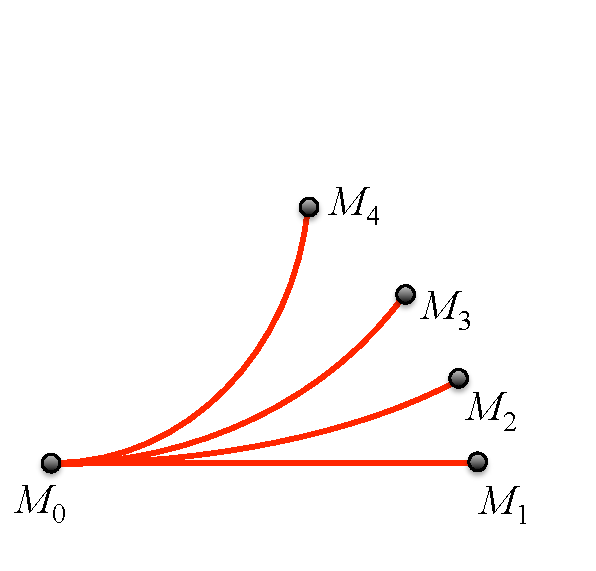
\includegraphics{./images/curves/c106.pdf}}}

				\vspace{-1em}\invisible<1->{{\b 长度相同的曲线,切线

				转角越大弯曲程度越大}}
			\end{center}
		\column{.5\textwidth}
	\end{columns}
\end{frame}

\begin{frame}{曲率}
	\linespread{1.2}
	\centerline{\ba{如何刻画曲线的弯曲程度?}}

	\begin{columns}
		\column{.5\textwidth}
			\begin{center}
				\vspace{-1em}
				{\resizebox{!}{5.5cm}{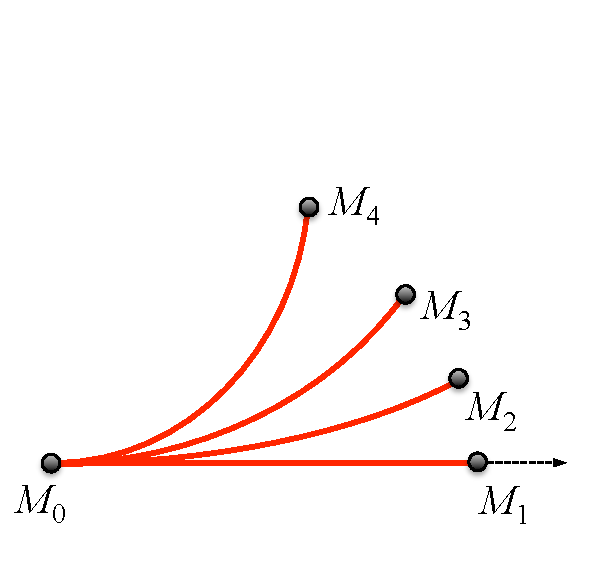
\includegraphics{./images/curves/c105.pdf}}}

				\vspace{-1em}\invisible<1->{{\b 长度相同的曲线,切线

				转角越大弯曲程度越大}}
			\end{center}
		\column{.5\textwidth}
	\end{columns}
\end{frame}

\begin{frame}{曲率}
	\linespread{1.2}
	\centerline{\ba{如何刻画曲线的弯曲程度?}}

	\begin{columns}
		\column{.5\textwidth}
			\begin{center}
				\vspace{-1em}
				{\resizebox{!}{5.5cm}{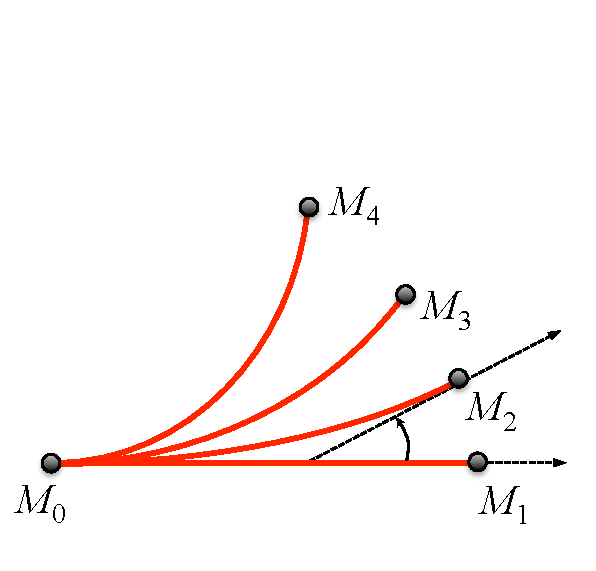
\includegraphics{./images/curves/c104.pdf}}}

				\vspace{-1em}\invisible<1->{{\b 长度相同的曲线,切线

				转角越大弯曲程度越大}}
			\end{center}
		\column{.5\textwidth}
	\end{columns}
\end{frame}

\begin{frame}{曲率}
	\linespread{1.2}
	\centerline{\ba{如何刻画曲线的弯曲程度?}}

	\begin{columns}
		\column{.5\textwidth}
			\begin{center}
				\vspace{-1em}
				{\resizebox{!}{5.5cm}{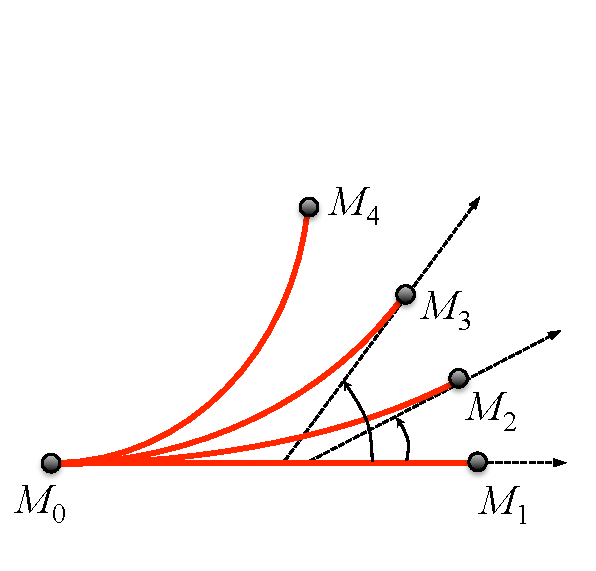
\includegraphics{./images/curves/c103.pdf}}}

				\vspace{-1em}\invisible<1->{{\b 长度相同的曲线,切线

				转角越大弯曲程度越大}}
			\end{center}
		\column{.5\textwidth}
	\end{columns}
\end{frame}

\begin{frame}{曲率}
	\linespread{1.2}
	\centerline{\ba{如何刻画曲线的弯曲程度?}}

	\begin{columns}
		\column{.5\textwidth}
			\begin{center}
				\vspace{-1em}
				{\resizebox{!}{5.5cm}{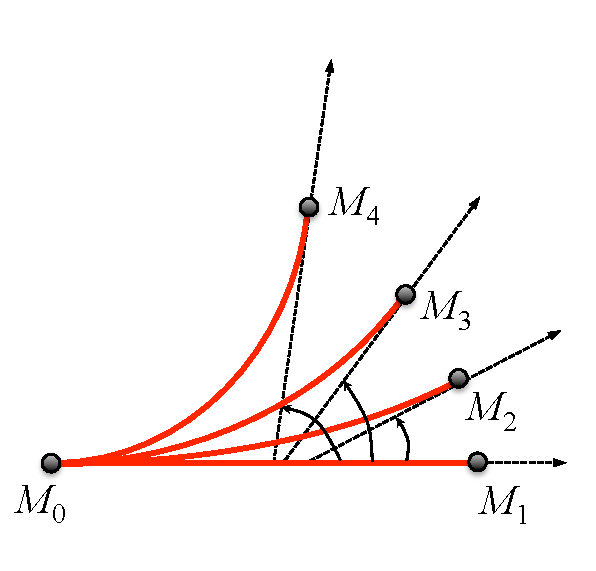
\includegraphics{./images/curves/c102.pdf}}}

				\vspace{-1em}\invisible<1->{{\b 长度相同的曲线,切线

				转角越大弯曲程度越大}}
			\end{center}
		\column{.5\textwidth}
	\end{columns}
\end{frame}

\begin{frame}{曲率}
	\linespread{1.2}
	\centerline{\ba{如何刻画曲线的弯曲程度?}}

	\begin{columns}
		\column{.5\textwidth}
			\begin{center}
				\vspace{-1em}
				{\resizebox{!}{5.5cm}{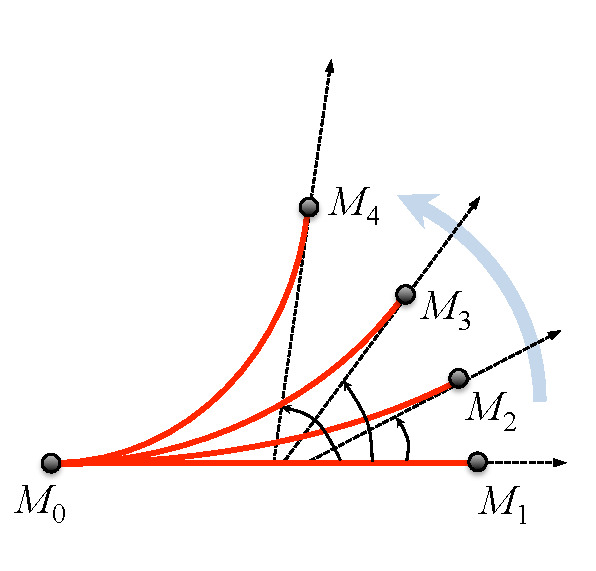
\includegraphics{./images/curves/c101.pdf}}}

				\vspace{-1em}{{\b 长度相同的曲线,切线

				转角越大弯曲程度越大}}
			\end{center}
		\column{.5\textwidth}
	\end{columns}
\end{frame}

% \begin{frame}{曲率}
% 	\linespread{1.2}
% 	\centerline{\ba{如何刻画曲线的弯曲程度?}}
% 
% 	\begin{columns}
% 		\column{.5\textwidth}
% 			\begin{center}
% 				\vspace{-1em}
% 				{\resizebox{!}{5.5cm}{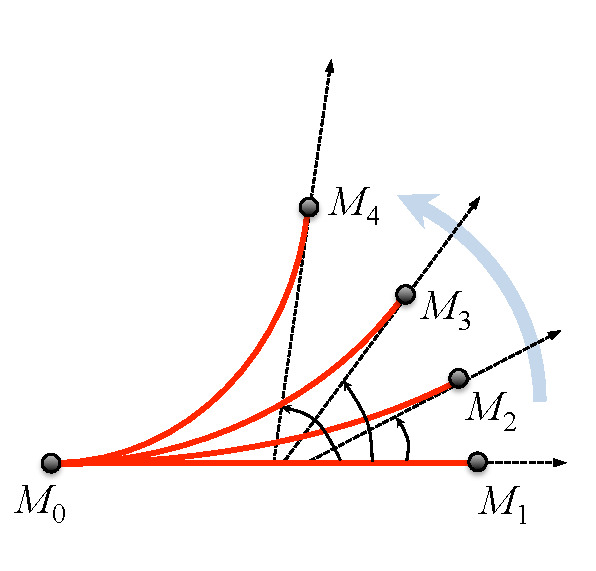
\includegraphics{./images/curves/c101.pdf}}}
% 
% 				\vspace{-1em}{{\b 长度相同的曲线,切线
% 				
% 				转角越大弯曲程度越大}}	
% 			\end{center}
% 		\column{.5\textwidth}
% 			\begin{center}			
% 				\vspace{-1em}
% 				{\resizebox{!}{5.5cm}{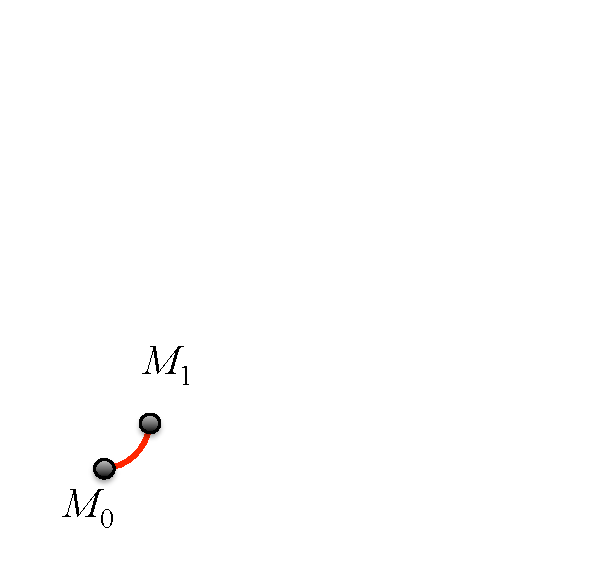
\includegraphics{./images/curves/c208.pdf}}}
% 				
% 				\vspace{-1em}{\color{white} 切线转角相同的曲线,
% 
% 				弧长越短弯曲程度越大}
% 			\end{center}
% 	\end{columns}
% \end{frame}
% 
% \begin{frame}{曲率}
% 	\linespread{1.2}
% 	\centerline{\ba{如何刻画曲线的弯曲程度?}}
% 
% 	\begin{columns}
% 		\column{.5\textwidth}
% 			\begin{center}
% 				\vspace{-1em}
% 				{\resizebox{!}{5.5cm}{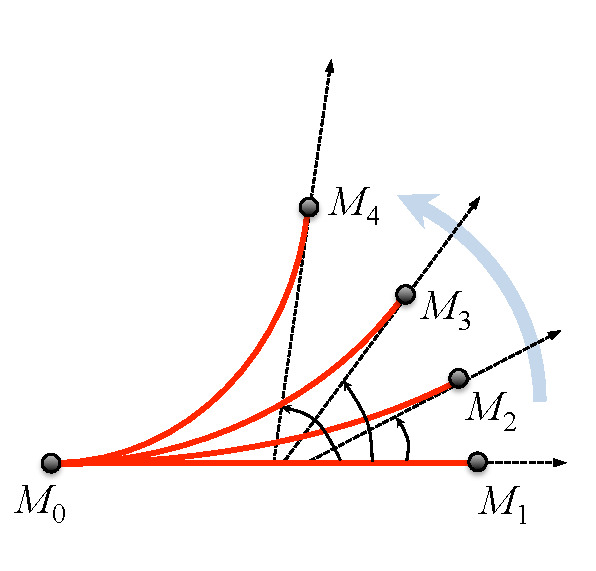
\includegraphics{./images/curves/c101.pdf}}}
% 
% 				\vspace{-1em}{{\b 长度相同的曲线,切线
% 
% 				转角越大弯曲程度越大}}
% 			\end{center}
% 		\column{.5\textwidth}
% 			\begin{center}
% 				\vspace{-1em}
% 				{\resizebox{!}{5.5cm}{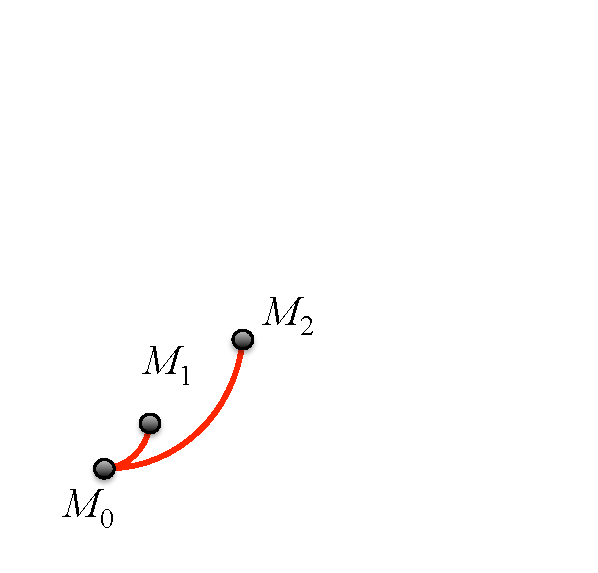
\includegraphics{./images/curves/c207.pdf}}}
% 				
% 				\vspace{-1em}{\color{white} 切线转角相同的曲线,
% 
% 				弧长越短弯曲程度越大}
% 			\end{center}
% 	\end{columns}
% \end{frame}

\begin{frame}{曲率}
	\linespread{1.2}
	\centerline{\ba{如何刻画曲线的弯曲程度?}}

	\begin{columns}
		\column{.5\textwidth}
			\begin{center}
				\vspace{-1em}
				{\resizebox{!}{5.5cm}{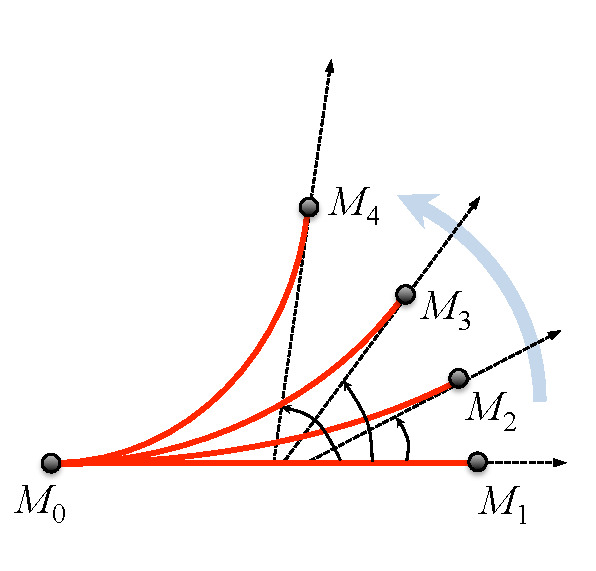
\includegraphics{./images/curves/c101.pdf}}}

				\vspace{-1em}{{\b 长度相同的曲线,切线

				转角越大弯曲程度越大}}
			\end{center}
		\column{.5\textwidth}
			\begin{center}
				\vspace{-1em}
				{\resizebox{!}{5.5cm}{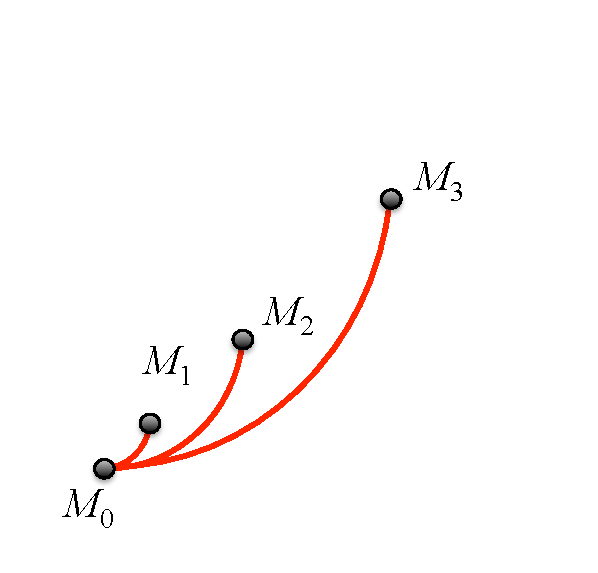
\includegraphics{./images/curves/c206.pdf}}}
				
				\vspace{-1em}{\color{white} 切线转角相同的曲线,

				弧长越短弯曲程度越大}
			\end{center}
	\end{columns}
\end{frame}

\begin{frame}{曲率}
	\linespread{1.2}
	\centerline{\ba{如何刻画曲线的弯曲程度?}}

	\begin{columns}
		\column{.5\textwidth}
			\begin{center}
				\vspace{-1em}
				{\resizebox{!}{5.5cm}{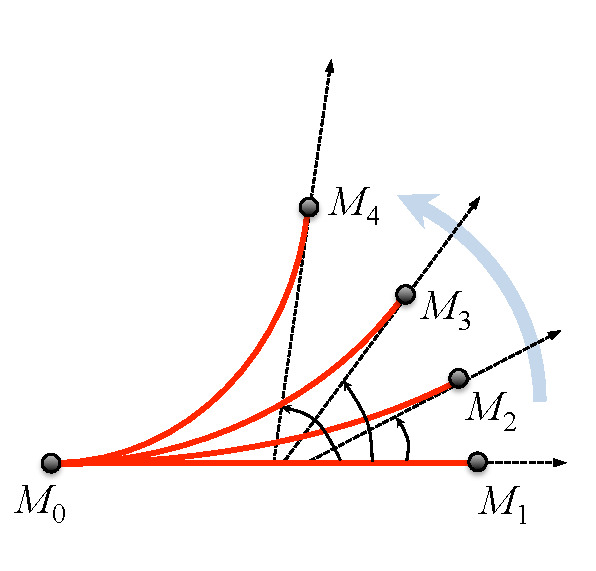
\includegraphics{./images/curves/c101.pdf}}}

				\vspace{-1em}{{\b 长度相同的曲线,切线

				转角越大弯曲程度越大}}
			\end{center}
		\column{.5\textwidth}
			\begin{center}
				\vspace{-1em}
				{\resizebox{!}{5.5cm}{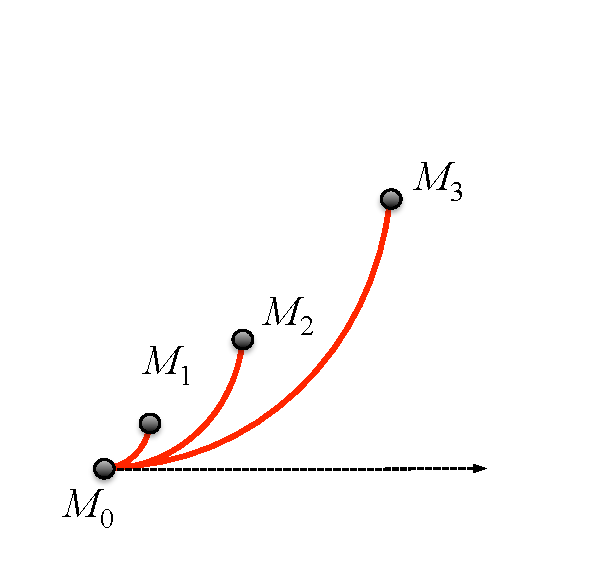
\includegraphics{./images/curves/c205.pdf}}}
				
				\vspace{-1em}{\color{white} 切线转角相同的曲线,

				弧长越短弯曲程度越大}
			\end{center}
	\end{columns}
\end{frame}

\begin{frame}{曲率}
	\linespread{1.2}
	\centerline{\ba{如何刻画曲线的弯曲程度?}}

	\begin{columns}
		\column{.5\textwidth}
			\begin{center}
				\vspace{-1em}
				{\resizebox{!}{5.5cm}{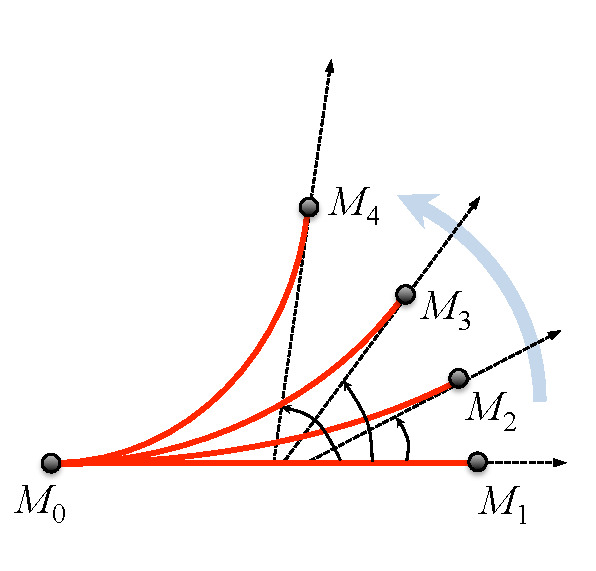
\includegraphics{./images/curves/c101.pdf}}}

				\vspace{-1em}{{\b 长度相同的曲线,切线

				转角越大弯曲程度越大}}
			\end{center}
		\column{.5\textwidth}
			\begin{center}
				\vspace{-1em}
				{\resizebox{!}{5.5cm}{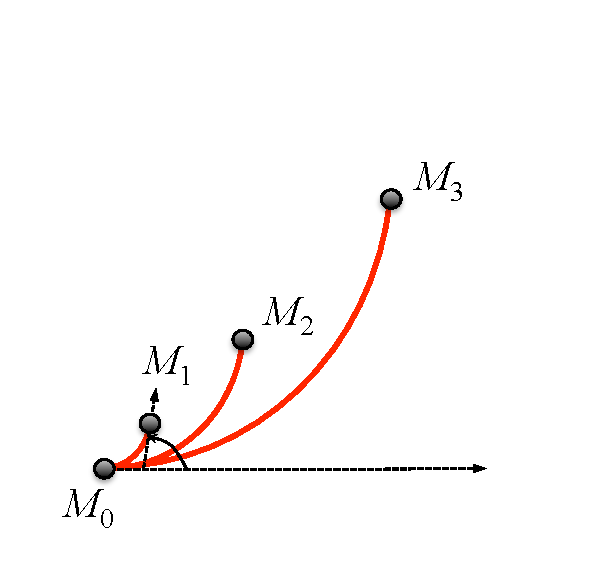
\includegraphics{./images/curves/c204.pdf}}}
				
				\vspace{-1em}{\color{white} 切线转角相同的曲线,

				弧长越短弯曲程度越大}
			\end{center}
	\end{columns}
\end{frame}

\begin{frame}{曲率}
	\linespread{1.2}
	\centerline{\ba{如何刻画曲线的弯曲程度?}}

	\begin{columns}
		\column{.5\textwidth}
			\begin{center}
				\vspace{-1em}
				{\resizebox{!}{5.5cm}{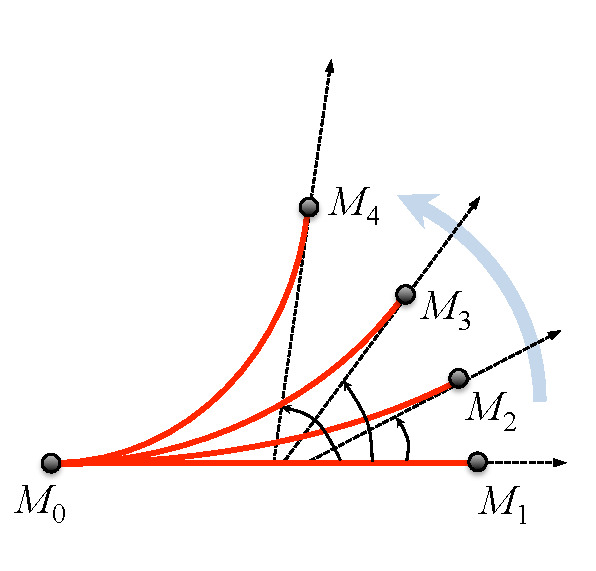
\includegraphics{./images/curves/c101.pdf}}}

				\vspace{-1em}{{\b 长度相同的曲线,切线

				转角越大弯曲程度越大}}
			\end{center}
		\column{.5\textwidth}
			\begin{center}
				\vspace{-1em}
				{\resizebox{!}{5.5cm}{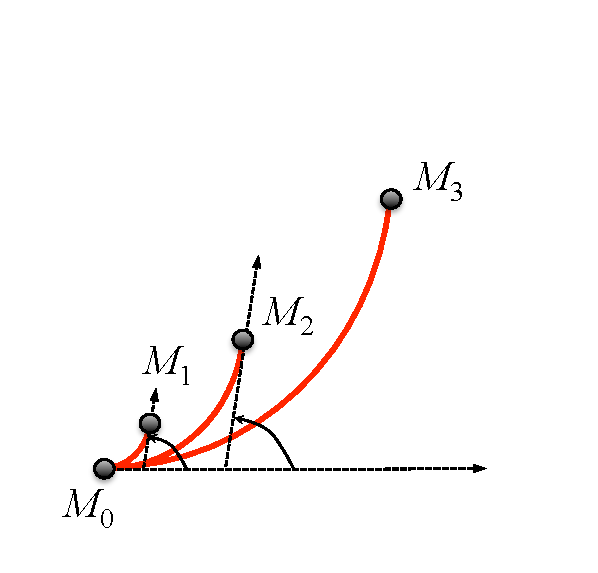
\includegraphics{./images/curves/c203.pdf}}}
				
				\vspace{-1em}{\color{white} 切线转角相同的曲线,

				弧长越短弯曲程度越大}
			\end{center}
	\end{columns}
\end{frame}

\begin{frame}{曲率}
	\linespread{1.2}
	\centerline{\ba{如何刻画曲线的弯曲程度?}}

	\begin{columns}
		\column{.5\textwidth}
			\begin{center}
				\vspace{-1em}
				{\resizebox{!}{5.5cm}{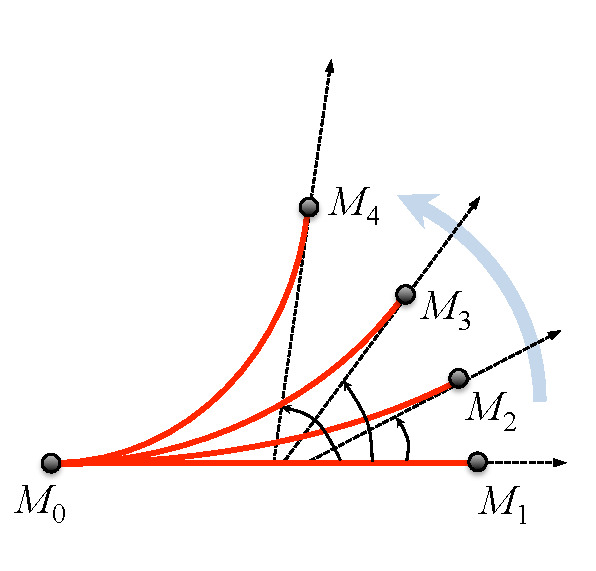
\includegraphics{./images/curves/c101.pdf}}}

				\vspace{-1em}{{\b 长度相同的曲线,切线

				转角越大弯曲程度越大}}
			\end{center}
		\column{.5\textwidth}
			\begin{center}
				\vspace{-1em}
				{\resizebox{!}{5.5cm}{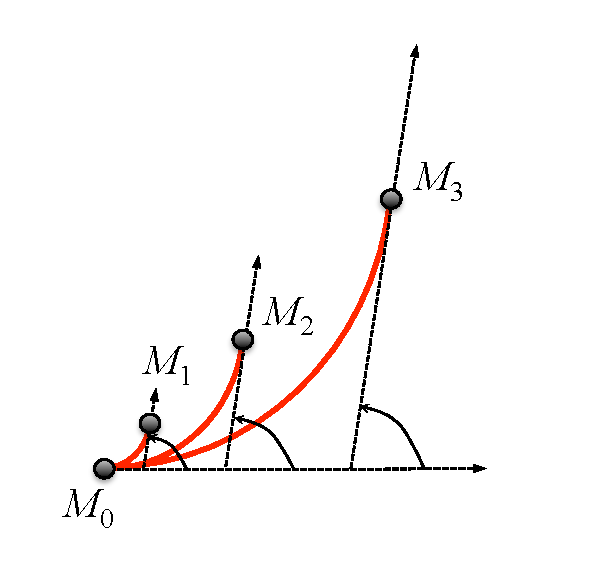
\includegraphics{./images/curves/c202.pdf}}}
				
				\vspace{-1em}{\color{white} 切线转角相同的曲线,

				弧长越短弯曲程度越大}
			\end{center}
	\end{columns}
\end{frame}

\begin{frame}{曲率}
	\linespread{1.2}
	\centerline{\ba{如何刻画曲线的弯曲程度?}}

	\begin{columns}
		\column{.5\textwidth}
			\begin{center}
				\vspace{-1em}
				{\resizebox{!}{5.5cm}{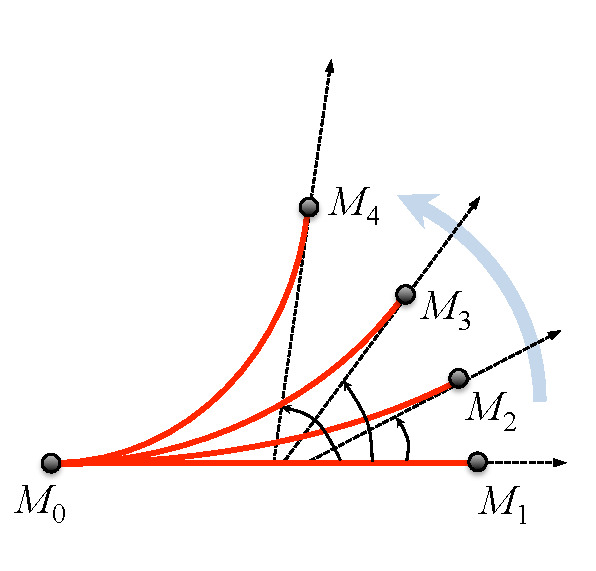
\includegraphics{./images/curves/c101.pdf}}}

				\vspace{-1em}{{\b 长度相同的曲线,切线

				转角越大弯曲程度越大}}
			\end{center}
		\column{.5\textwidth}
			\begin{center}
				\vspace{-1em}
				{\resizebox{!}{5.5cm}{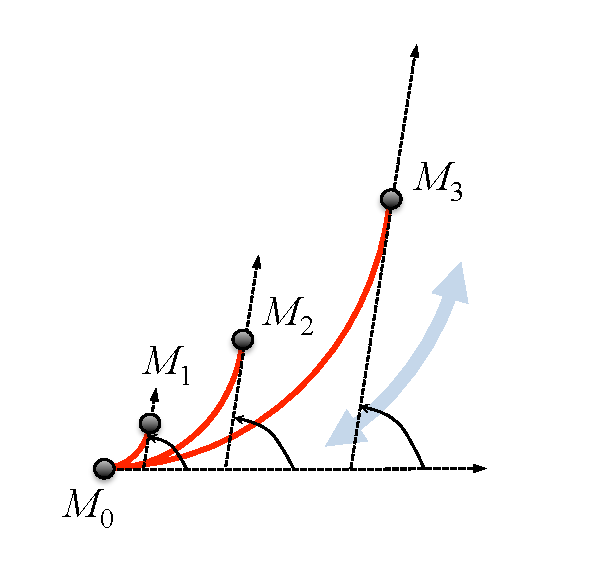
\includegraphics{./images/curves/c201.pdf}}}
				
				\vspace{-1em}{\b 切线转角相同的曲线,

				弧长越短弯曲程度越大}
			\end{center}
	\end{columns}
\end{frame}

%=================================================

\begin{frame}{1、曲率的定义}
	\linespread{1.5}
	\ba{曲线的弯曲程度与切线的转角成正比,弧长成反比}\pause
	\begin{block}{{\bf 定义1}\hfill }
		设曲线$C:y=f(x)$光滑且可求长度,从其上一点$M_0$出发,
		到另一点$M$的弧长
		为$\Delta s$,切线转角为$\Delta\alpha$。
		\pause 若
		
		极限$\lim\limits_{\Delta s\to
		0}\left|\df{\Delta\alpha}{\Delta s}\right|$存在,
		则称之为{\bb 曲线$C$在$M_0$处的曲率},记为
	$$\alert{K=\lim\limits_{\Delta s\to
				0}\left|\df{\Delta\alpha}{\Delta s}\right|\pause
				=\left|\df{d\alpha}{ds}\right|}$$ 
	\end{block}
% 	\pause 
% 	\begin{itemize}
% 	  \item \alert{曲率:曲线切线转角关于弧长的变化率}
% 	\end{itemize}
\end{frame}

\subsection{曲率的计算}

\begin{frame}{2、曲率的计算}
	\linespread{1.2}\pause 
	设$y=f(x)$二阶可导,则
	\alert{$$K=\left|\df{d\alpha}{ds}\right|
				\pause =\df{|y''|}{[1+(y')^2]^{3/2}}$$}\pause 
	\begin{exampleblock}{{\bf 例1}\hfill }
		求椭圆$x=3\cos \theta,y=2\sin \theta\,(0\leq \theta\leq 2\pi)$
		上任意点处的曲率,并指出其中曲率最大的点。
	\end{exampleblock} 
\end{frame}

\begin{frame}
	\linespread{1.2}
	\alert{{\bf 注:}根据不同形式的曲线方程,可以得到相应的曲率公式}\pause 
	\begin{enumerate}
	  \item 若曲线由参数方程$\left\{\begin{array}{l}
	  x=\varphi(t)\\ y=\psi(t)
	  \end{array}\right.$给出,\pause 则
	  $$\alert{K=\df{|\varphi'(t)\psi''(t)-\varphi''(t)\psi'(t)|}
		{\{[\varphi'(t)]^2+[\psi'(t)]^2\}^{3/2}}}$$\pause 
	  \item 若曲线方程为$x=g(y)$,\pause 则
		$$\alert{K=\df{|g''(y)|}{\{[1+[g'(y)]^2\}^{3/2}}}$$
	\end{enumerate}
\end{frame}

\subsection{曲率圆与曲率的应用}

\begin{frame}{3、曲率圆与曲率的应用}
	\linespread{1.2} \pause 
	{\bb 曲率圆:}与已知曲线在凹侧相切,且曲率相同的圆
	
	\pause\vspace{1ex}
	\begin{center}
		\resizebox{!}{4cm}{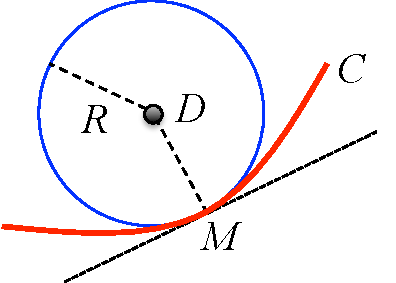
\includegraphics{./images/curSphere.pdf}}
	\end{center}
	\vspace{-1em}\pause 
	\begin{block}{\bf 定理1}
		曲率圆与给定曲线二阶相切。
	\end{block}
% 	\pause {\bb 曲率半径:}\hspace{3cm}{$\alert{R=\df 1K}$}
\end{frame}

\begin{frame}
	\linespread{1.2} 
	\begin{exampleblock}{{\bf 例2}(加工问题)\hfill }
		已知某工件内侧的截痕曲线为椭圆$\df{x^2}9+\df{y^2}4=1$,
		若用圆形砂轮对其进行打磨,问该如何选择砂轮的尺寸?
	\end{exampleblock}
	\vspace{-1em}
	\begin{columns}
		\column{.55\textwidth}
			\begin{center}
				\only<1>{\resizebox{!}{5.5cm}{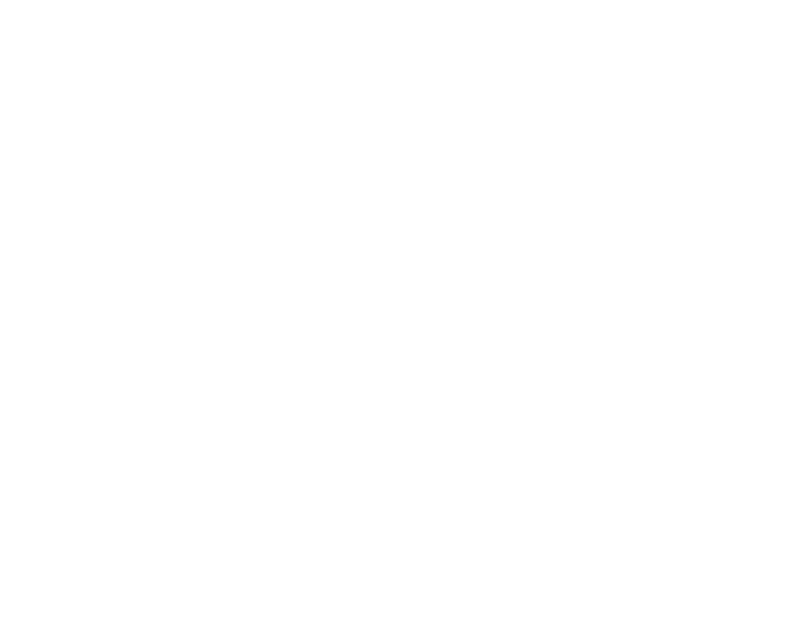
\includegraphics{./images/SE/S0x.pdf}}}%
				\only<2>{\resizebox{!}{5.5cm}{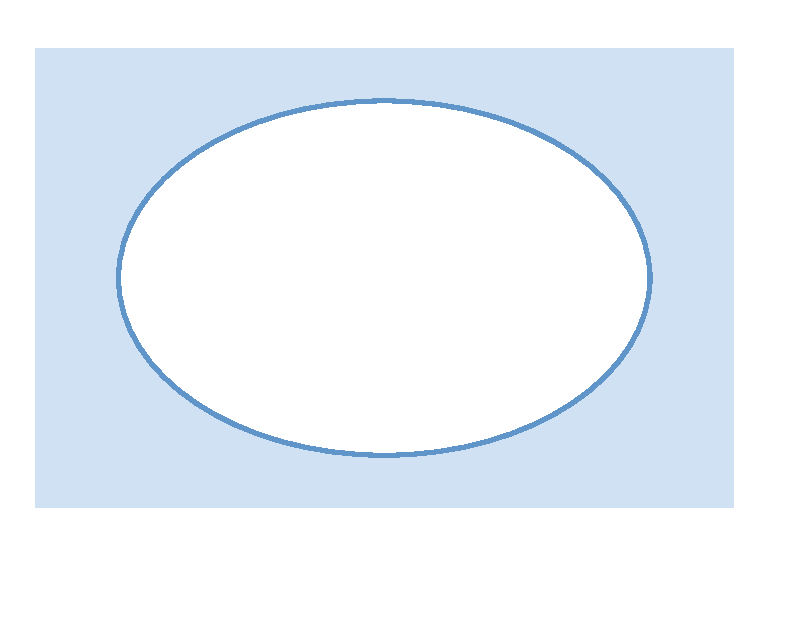
\includegraphics{./images/SE/S05.pdf}}}%
				\only<3-4>{\resizebox{!}{5.5cm}{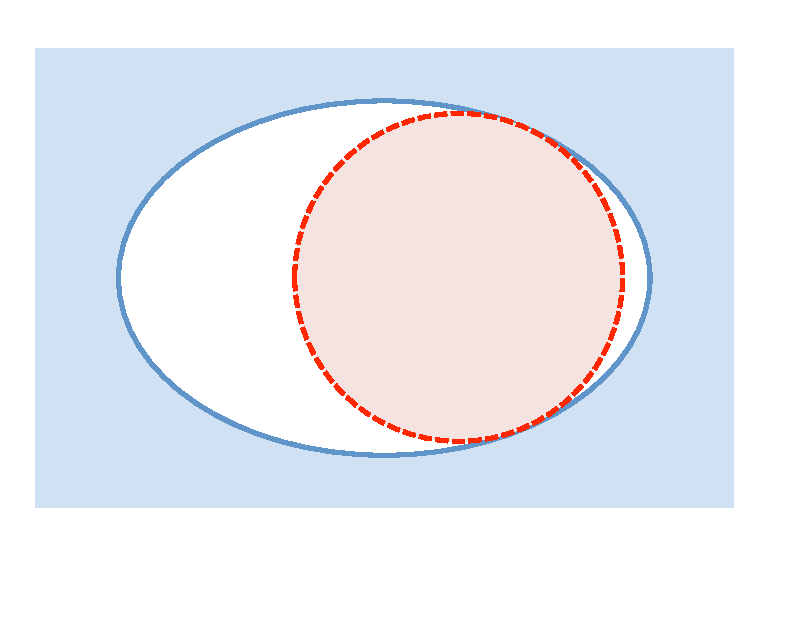
\includegraphics{./images/SE/S04.pdf}}}%
				\only<5-6>{\resizebox{!}{5.5cm}{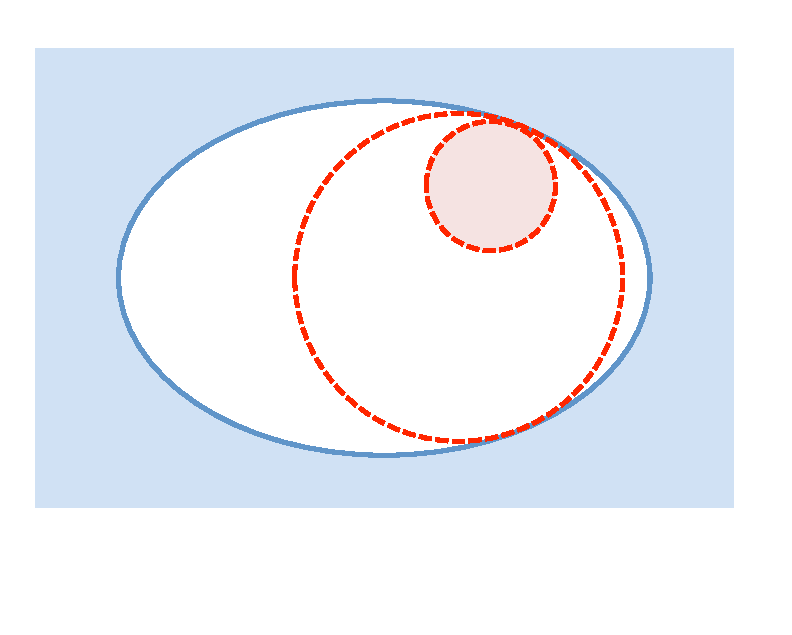
\includegraphics{./images/SE/S03.pdf}}}%
				\only<7-8>{\resizebox{!}{5.5cm}{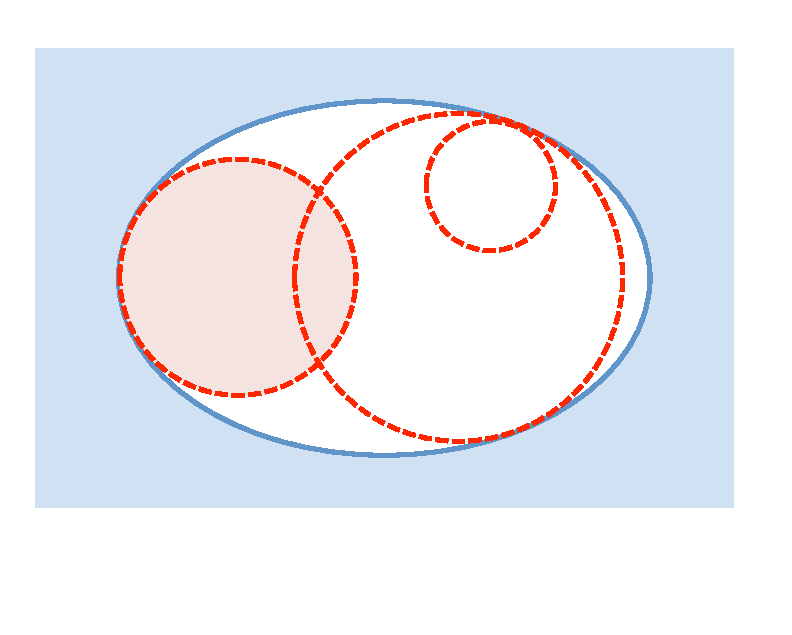
\includegraphics{./images/SE/S02.pdf}}}%
				\only<9>{\resizebox{!}{5.5cm}{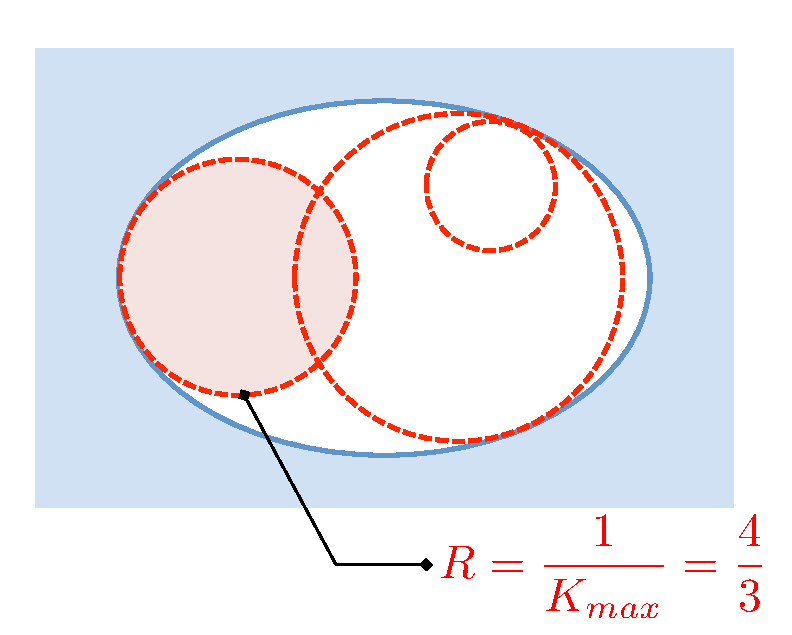
\includegraphics{./images/SE/S01.pdf}}}%
			\end{center}
		\column{.45\textwidth}
%  			{\bf 分析:}
			\begin{itemize}
			  \item<4-> 半径过大$\Rightarrow$无法完全打磨
			  \item<6-> 半径过小$\Rightarrow$打磨效率过低
			  \item<8-> {\bf 最优解:}\alert{半径最小的曲率圆}
			\end{itemize}
	\end{columns}
\end{frame}

\begin{frame}{曲率半径与离心力}
	\linespread{1.2}
	\begin{columns}
		\column{.6\textwidth}
			质量为$m$的质点以速度$v$通过光滑曲线上一点,所受离心力为
			$$F=\df{mv^2}{R},$$
			其中$R$为曲线在该点处的曲率半径。
		\column{.4\textwidth}
			\begin{center}
				\resizebox{!}{4.5cm}{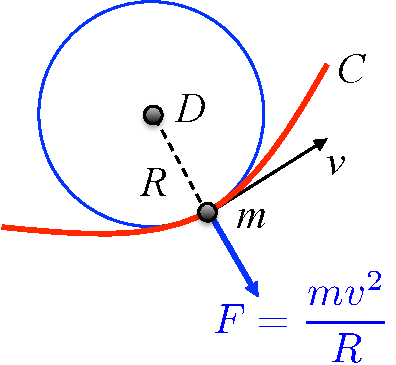
\includegraphics{./images/flip.pdf}}
			\end{center}
	\end{columns}
% 	\begin{exampleblock}{{\bf 例3}\hfill}
% 		飞机沿抛物线$y=\df{x^2}{4000}$(单位:m)俯冲,在最低点处
% 		速度为$v=400$m/s。飞行员体重$70$kg,求在最低点处飞行员
% 		对座椅的压力。(设重力加速度$g=10$N/kg)
% 	\end{exampleblock}
\end{frame}

% \begin{frame}
% 	\linespread{1.2}
% 	\begin{exampleblock}{{\bf 例3}\hfill}
% 		飞机沿抛物线$y=\df{x^2}{4000}$(单位:m)俯冲,在最低点处
% 		速度为$v=400$m/s。飞行员体重$70$kg,求在最低点处飞行员
% 		对座椅的压力。(设重力加速度$g=10$m/s$^2$)
% 	\end{exampleblock}
% 	\pause 
% 	\begin{columns}
% 		\column{.6\textwidth}
% 			\begin{center}
% 				\resizebox{!}{4.5cm}{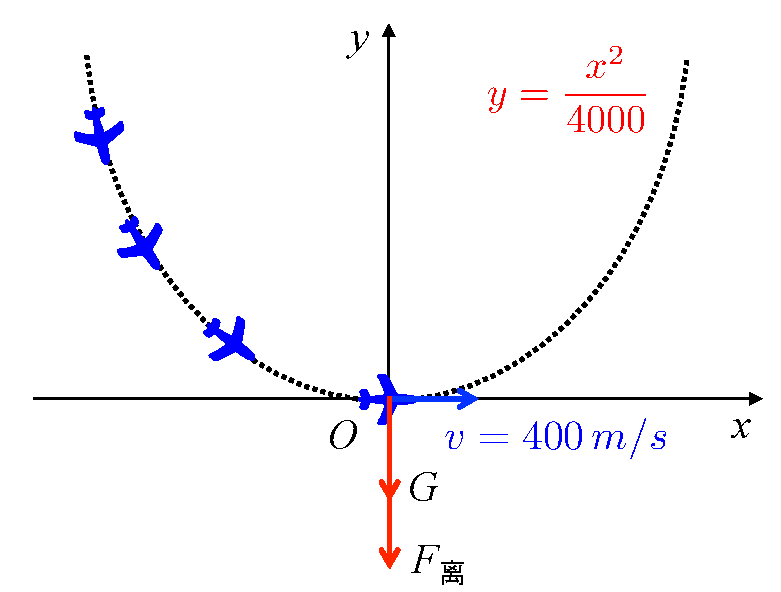
\includegraphics{./images/ac.pdf}}
% 			\end{center}
% 		\column{.4\textwidth}\pause 
% % 			{\bf 解:}抛物线在最低点处的曲率半径
% % 			$$R=\df 1K=2\,(km),$$
% % 			故所求压力
% 			\begin{eqnarray*}
% 				F & = & G+F_{\mbox{离}}\pause \\
% 				& = & mg\pause +\df{mv^2}R\pause \\
% 				& = & mg +mv^2K\pause \\
% 				& = & 6300\;(N)
% 			\end{eqnarray*}
% 	\end{columns}
% \end{frame}

\begin{frame}{铁路中的缓和曲线}
	\linespread{1.2}\pause
	\begin{columns}
		\column{.2\textwidth}
			\begin{center}
				\resizebox{!}{1.2cm}{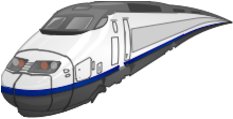
\includegraphics{./images/train.pdf}}
			\end{center}
		\column{.8\textwidth}
			\ba{为了确保列车行驶安全,尽可能保证列车运行时所受离心力的平稳变化。}\pause 
	\end{columns} 
	\vspace{-1em}
	\begin{columns}
		\column{.65\textwidth}
			\begin{center}
				\only<1-2>{\resizebox{!}{5.5cm}{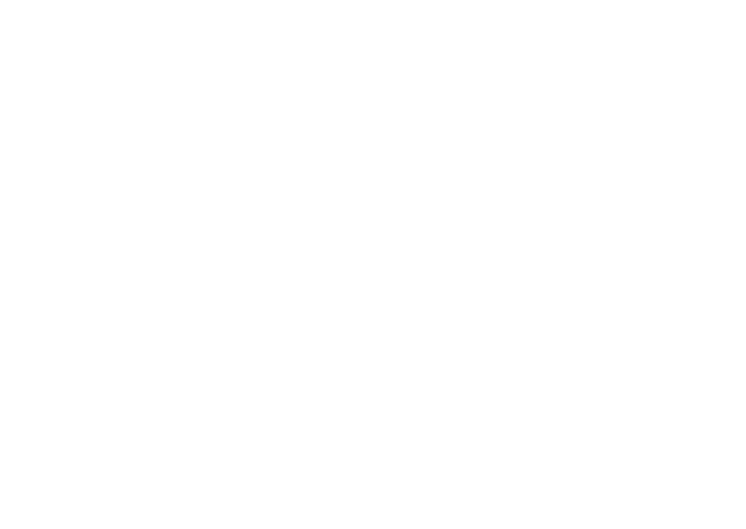
\includegraphics{./images/rc00.pdf}}}%
				\only<3-8>{\resizebox{!}{5.5cm}{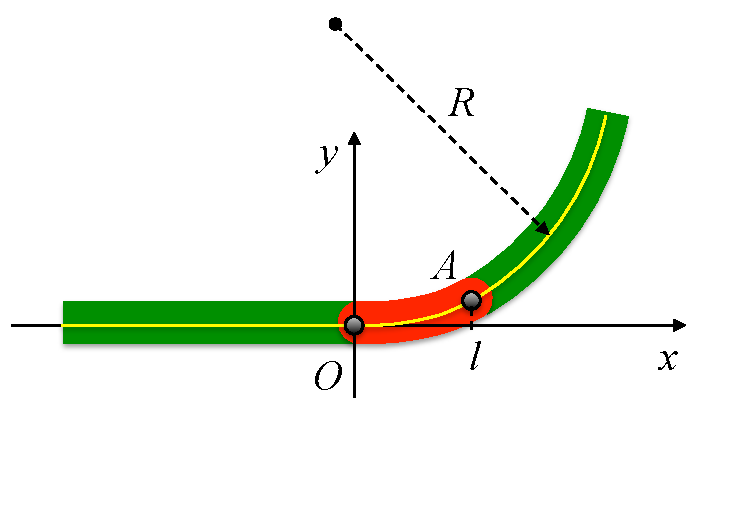
\includegraphics{./images/rc02.pdf}}}%
% 				\only<9>{\resizebox{!}{5.5cm}{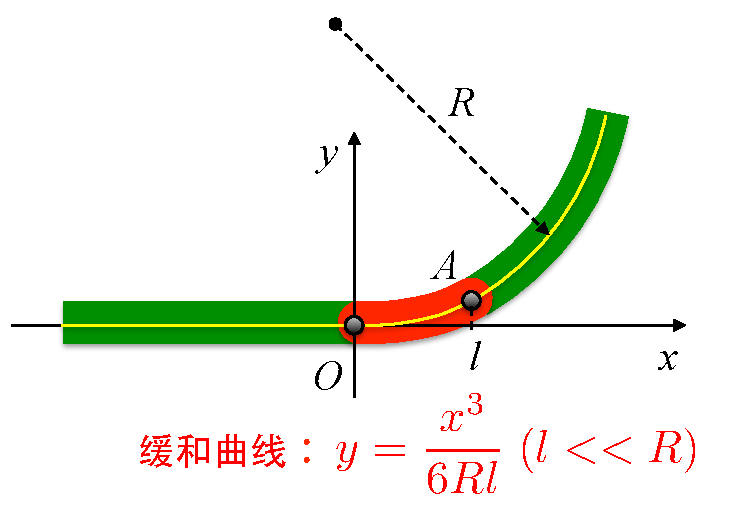
\includegraphics{./images/rc01.pdf}}}%
			\end{center}
		\column{.35\textwidth}
			\uncover<4->{\ba{常用的缓和曲线:}}%
			\begin{itemize}
			  \item<5-> {\b 三次多项式}
			  \item<6-> {\b 渐开螺旋线}
			  \item<7-> {\b 双扭线}
			  \item<8-> {\b \ldots}
			\end{itemize}
	\end{columns}
\end{frame}

\begin{frame}
	\linespread{1.2}
	\begin{exampleblock}{{\bf 例3}(铁路的缓和曲线)}
		如图,列车匀速行进,经过一段直线轨道后,将进入半径为$R$的圆弧轨道。为
		尽量减少列车行驶中所受的离心力冲击,
		试确定一个三次多项式函数实现两段轨道的连接。
	\end{exampleblock}
	\vspace{-1ex}
	\begin{center}
% 		\only<1>{\resizebox{!}{5.2cm}{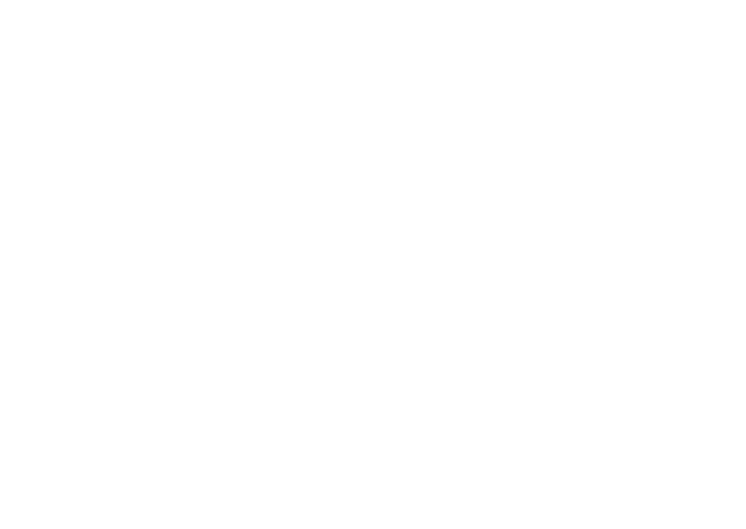
\includegraphics{./images/rc00.pdf}}}%
		\only<1>{\resizebox{!}{5.2cm}{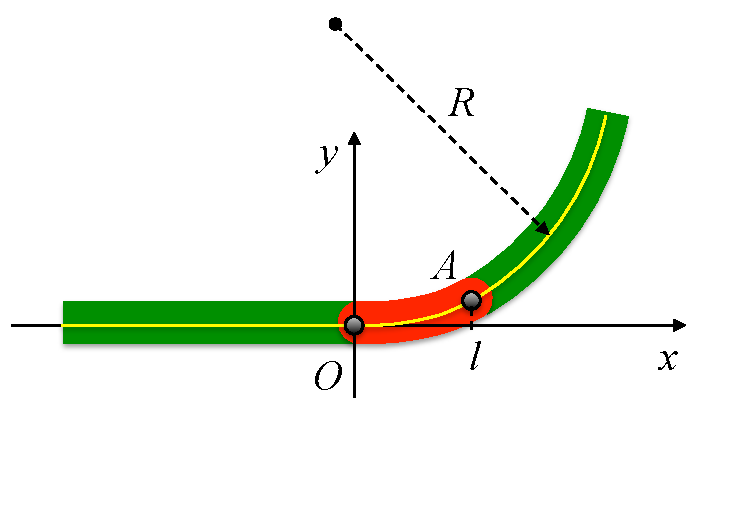
\includegraphics{./images/rc02.pdf}}}%
		\only<2>{\resizebox{!}{5.2cm}{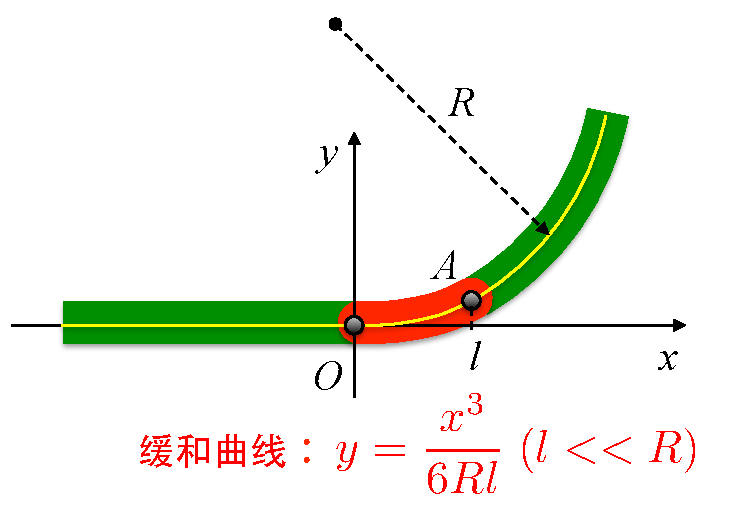
\includegraphics{./images/rc01.pdf}}}%
	\end{center}
\end{frame}

\begin{frame}
	\linespread{1}
	\begin{columns}
		\column{.55\textwidth}
			\resizebox{!}{4.5cm}{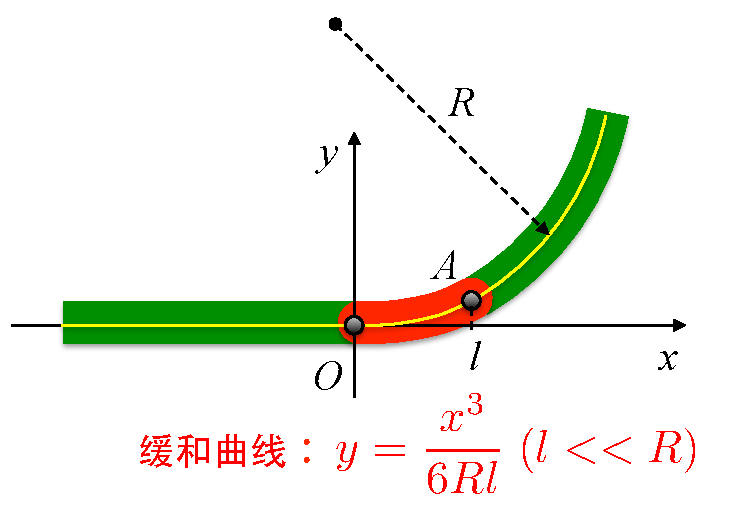
\includegraphics{./images/rc01.pdf}}
		\column{.45\textwidth}
			{\small
			\begin{itemize}
			  \item 匀速行驶$v=108km/h$
			  \item 乘客体重$m=50kg$
			  \item 圆弧半径$R=2000m$
			  \item 缓和曲线长$l=50m$
			\end{itemize}
			}
	\end{columns}
	\vspace{-1em}\pause
	\begin{columns}
		\column{.55\textwidth}
			\begin{center}
				\resizebox{!}{4cm}{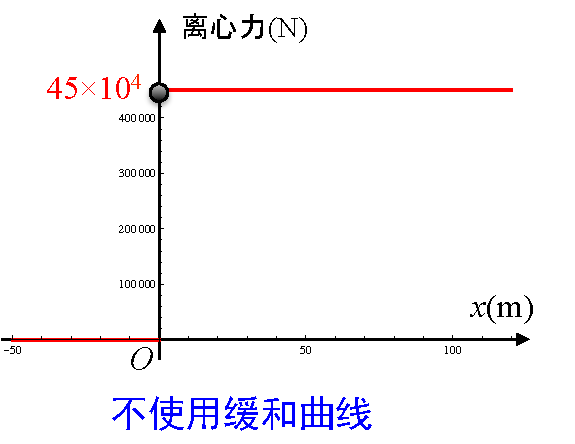
\includegraphics{./images/f01.pdf}}\pause
			\end{center}
		\column{.45\textwidth}
			\begin{center}
				\resizebox{!}{4cm}{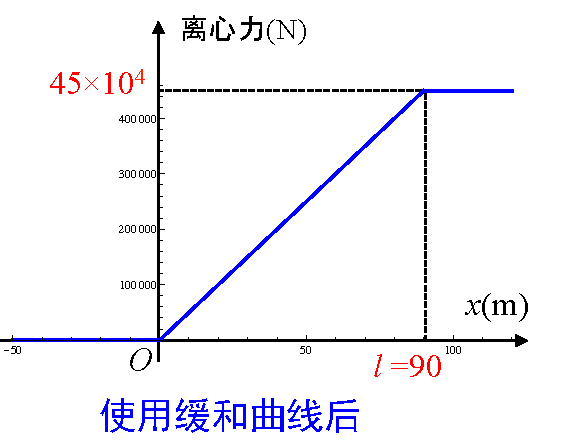
\includegraphics{./images/f02.pdf}}
			\end{center}
	\end{columns}
\end{frame}

\begin{frame}{铁路与轨道交通}
	\linespread{1.2}
	\vspace{-2em}
	\begin{center}
		\hspace{1em}\resizebox{!}{8cm}{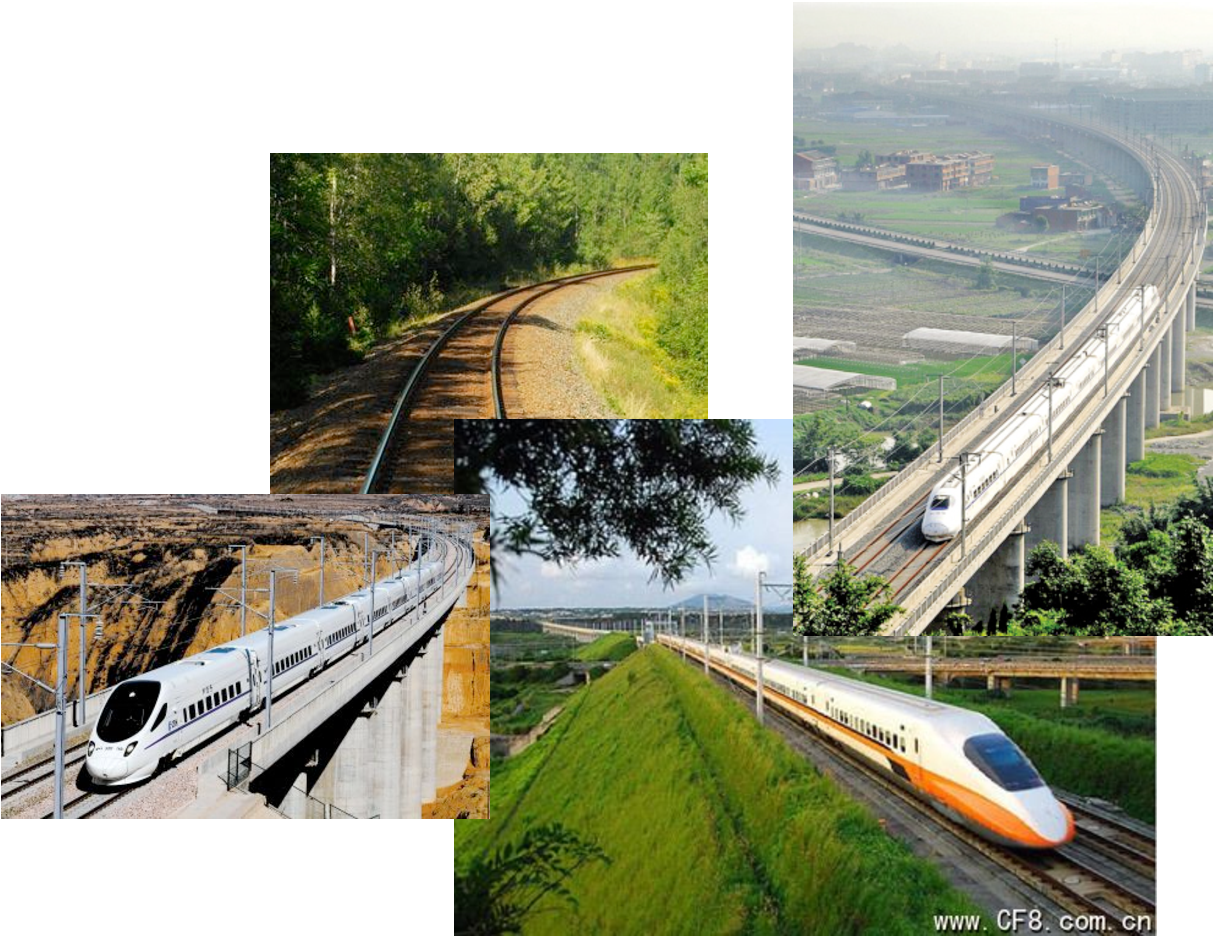
\includegraphics{./images/hr.pdf}}
	\end{center}
\end{frame}

\begin{frame}{高速公路}
	\linespread{1.2}
	\vspace{-1ex}
	\begin{center}
		\hspace{1em}\resizebox{!}{7.2cm}{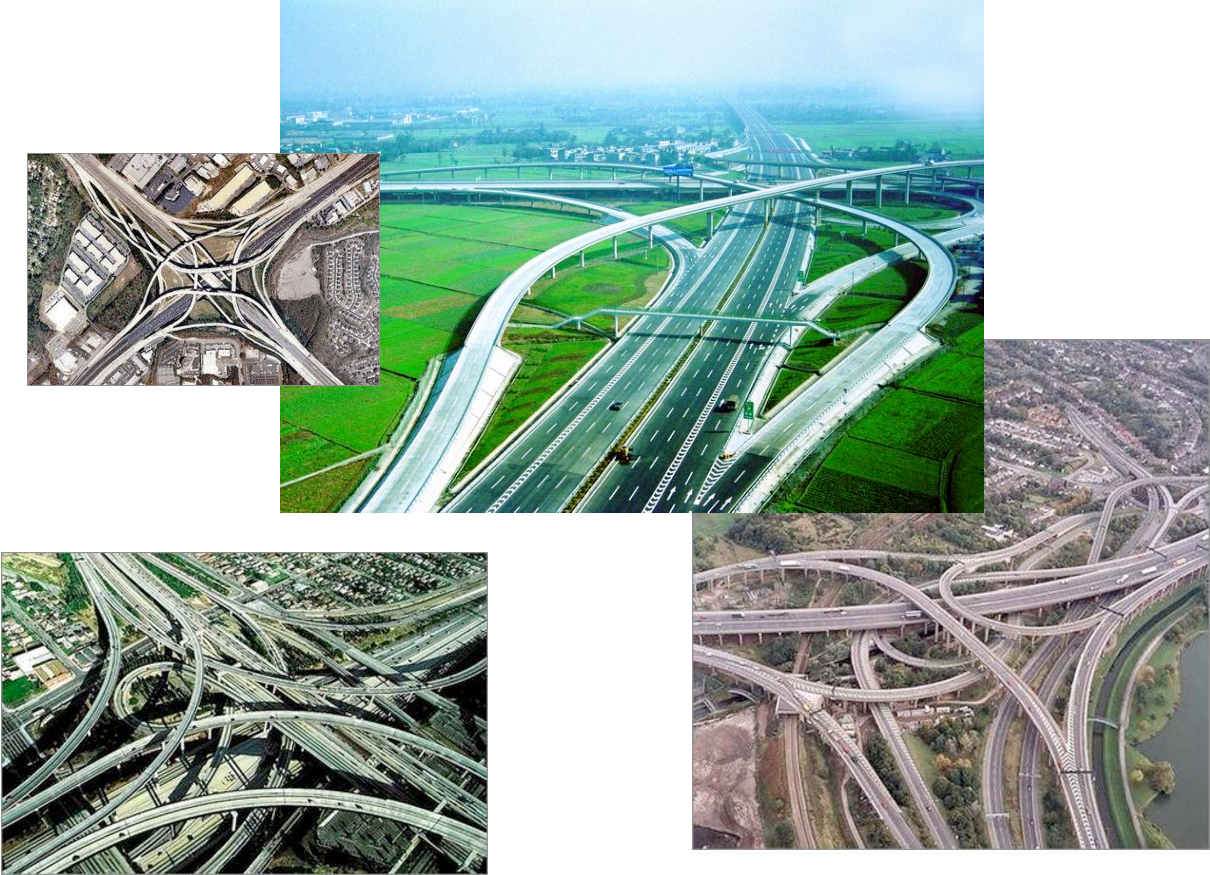
\includegraphics{./images/hw.pdf}}
	\end{center}
\end{frame}

\begin{frame}{过山车}
	\linespread{1.2}
	\vspace{-1ex}
	\begin{center}
		\hspace{1em}\resizebox{!}{7cm}{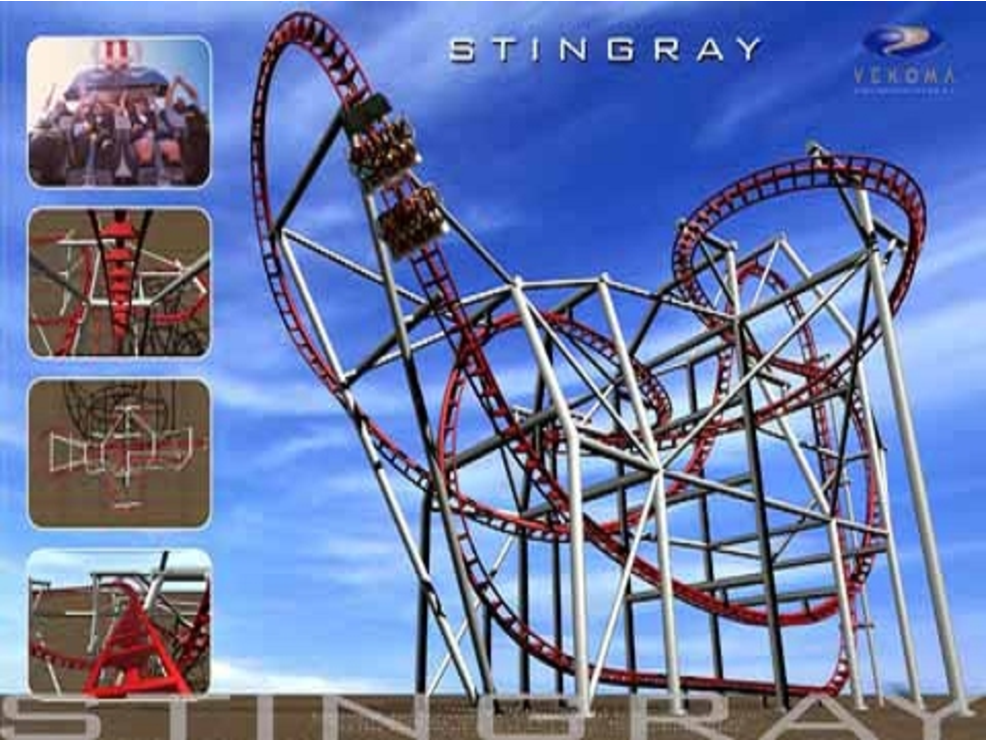
\includegraphics{./images/stg01.pdf}}
	\end{center}
\end{frame}

\begin{frame}{过山车}
	\linespread{1.2}
	\vspace{-1ex}
	\begin{center}
		\hspace{1em}\resizebox{!}{7.2cm}{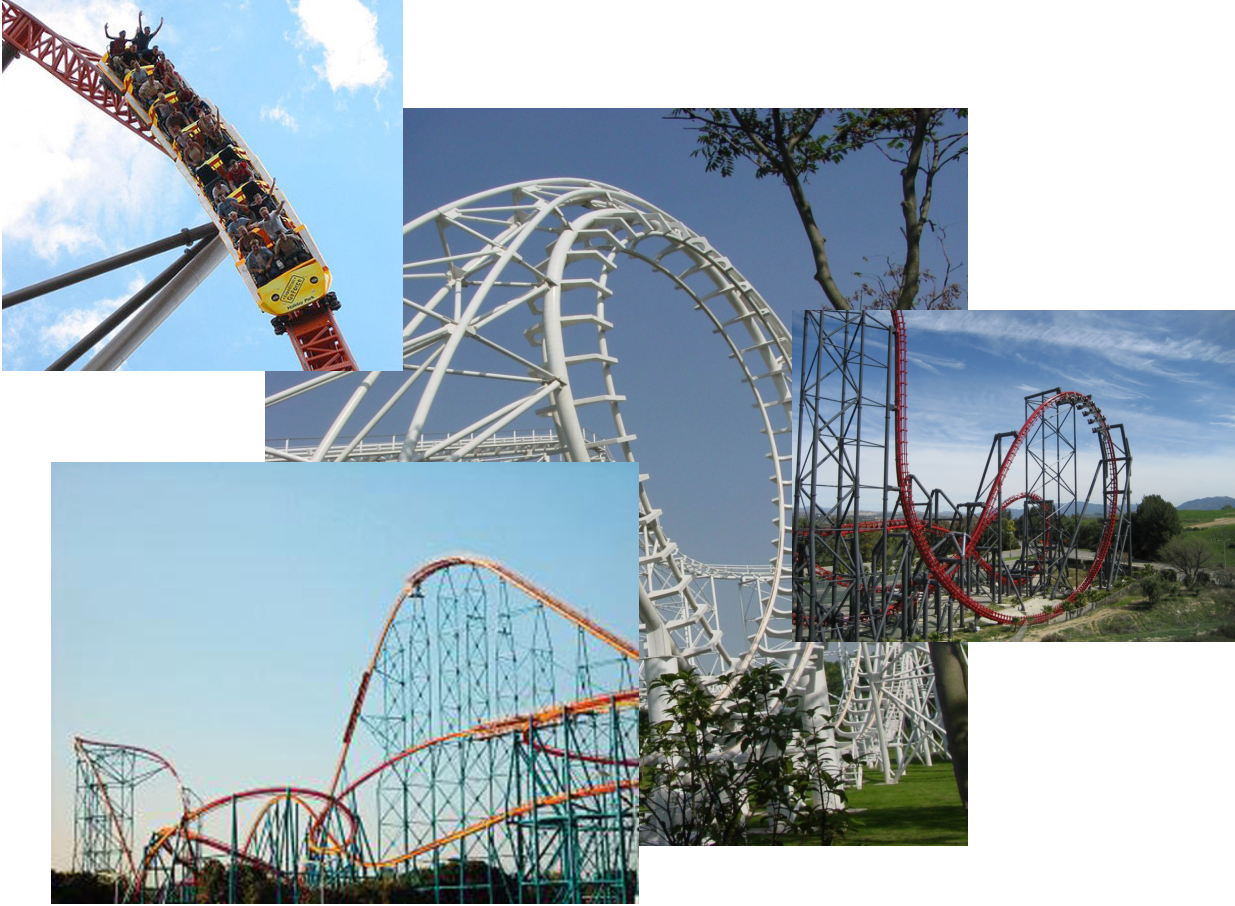
\includegraphics{./images/stg02.pdf}}
	\end{center}
\end{frame}

\begin{frame}{小结}
	\linespread{1.2}
	\begin{enumerate}
	  \item {\bf 曲率:}切线转角相对于弧长的变化率
	  \item {\bf 曲率的计算:}
	  $$\alert{K=\left|\df{d\alpha}{ds}\right|
				=\df{|y''|}{[1+(y')^2]^{3/2}}}$$
	  \item {\bf 曲率圆与曲率的应用}
	  \begin{itemize}
	    \item 曲率半径、离心力与缓和曲线
	  \end{itemize}
	\end{enumerate}
	\pause
	\begin{exampleblock}{{\bf 课后思考题}(过山车设计)\hfill}
		试设计一个分段的多项式函数,完成过山车上一段水平轨道与一段上坡直线轨道的接合。
	\end{exampleblock}
\end{frame}
